\documentclass[a4paper, 11pt]{article}
\usepackage{comment} % enables the use of multi-line comments (\ifx \fi) 
\usepackage{lipsum} %This package just generates Lorem Ipsum filler text. 
\usepackage{fullpage} % changes the margin
\usepackage[a4paper, total={7in, 10in}]{geometry}
\usepackage[fleqn]{amsmath}
\usepackage{amssymb,amsthm}  % assumes amsmath package installed
\newtheorem{theorem}{Theorem}
\newtheorem{corollary}{Corollary}
\usepackage{graphicx}
\usepackage{tikz}
\usetikzlibrary{arrows}
\usepackage{verbatim}
\usepackage[numbered]{mcode}
\usepackage{float}
\usepackage{tikz}
    \usetikzlibrary{shapes,arrows}
    \usetikzlibrary{arrows,calc,positioning}

    \tikzset{
        block/.style = {draw, rectangle,
            minimum height=1cm,
            minimum width=1.5cm},
        input/.style = {coordinate,node distance=1cm},
        output/.style = {coordinate,node distance=4cm},
        arrow/.style={draw, -latex,node distance=2cm},
        pinstyle/.style = {pin edge={latex-, black,node distance=2cm}},
        sum/.style = {draw, circle, node distance=1cm},
    }
\usepackage{xcolor}
\usepackage{mdframed}
\usepackage[shortlabels]{enumitem}
\usepackage{indentfirst}
\usepackage{hyperref}
    
\renewcommand{\thesubsection}{\thesection.\alph{subsection}}

\newenvironment{problem}[2][Problem]
    { \begin{mdframed}[backgroundcolor=gray!20] \textbf{#1 #2} \\}
    {  \end{mdframed}}

% Define solution environment
\newenvironment{solution}
    {\textit{Solution:}}
    {}

\renewcommand{\qed}{\quad\qedsymbol}
%%%%%%%%%%%%%%%%%%%%%%%%%%%%%%%%%%%%%%%%%%%%%%%%%%%%%%%%%%%%%%%%%%%%%%%%%%%%%%%%%%%%%%%%%%%%%%%%%%%%%%%%%%%%%%%%%%%%%%%%%%%%%%%%%%%%%%%%
\begin{document}
%Header-Make sure you update this information!!!!
\noindent
%%%%%%%%%%%%%%%%%%%%%%%%%%%%%%%%%%%%%%%%%%%%%%%%%%%%%%%%%%%%%%%%%%%%%%%%%%%%%%%%%%%%%%%%%%%%%%%%%%%%%%%%%%%%%%%%%%%%%%%%%%%%%%%%%%%%%%%%
\large\textbf{Shahid Beheshti University } \hfill \textbf{Homework - 1}   \\
%Email: veralevel@gethu.edu \hfill ID: 123456789 \\
\normalsize Course: CE 057 - Basic of Cryptography \hfill Term: Spring 2023\\
%Instructor: Dr. Raziyeh Salarifard \hfill Due Date: $22^{nd}$ November, 2019 \\
Instructor: Dr. Raziyeh Salarifard\\
\noindent\rule{7in}{2.8pt}

%%%%%%%%%%%%%%%%%%%%%%%%%%%%%%%%%%%%%%%%%%%%%%%%%%%%%%%%%%%%%%%%%%%%%%%%%
%Section 1
%%%%%%%%%%%%%%%%%%%%%%%%%%%%%%%%%%%%%%%%%%%%%%%%%%%%%%%%%%%%%%%%%%%%%%%%%%%%%%%%%%%%%%%%%%%%%%%%%%%%%%%%%%%%%%%%%%%%%%%%%%%%%%%%%%%%%%%%
% Problem 1
%%%%%%%%%%%%%%%%%%%%%%%%%%%%%%%%%%%%%%%%%%%%%%%%%%%%%%%%%%%%%%%%%%%%%%%%%%%%%%%%%%%%%%%%%%%%%%%%%%%%%%%%%%%%%%%%%%%%%%%%%%%%%%%%%%%%%%%%
\section*{Introduction to Cryptography}
\begin{problem}{1}
Let's start off with the fact that there are $n\cdot n$ ordered pairs of (person, person). Now we assume that nobody needs encryption to talk to themselves, so we subtract the $n$ pairs where the person is the same, to get $n\cdot n-n=n(n-1)$. Next, we note that the same secret key can be used to send messages on the route (A,B) as on the route (B,A) (with proper care taken to avoid reusing the same nonce, etc). So we divide by two to get $n(n-1)/2$. Finally, we plug in $n=20$ to get $20\cdot 19/2=10\cdot 19=190$.
\end{problem}

%%%%%%%%%%%%%%%%%%%%%%%%%%%%%%%%%%%%%%%%%%%%%%%%%%%%%%%%%%%%%%%%%%%%%%%%%
% Problem 2
%%%%%%%%%%%%%%%%%%%%%%%%%%%%%%%%%%%%%%%%%%%%%%%%%%%%%%%%%%%%%%%%%%%%%%%%%%%%%%%%%%%%%%%%%%%%%%%%%%%%%%%%%%%%%%%%%%%%%%%%%%%%%%%%%%%%%%%%
\begin{problem}{2}
a. Each of 8 letters can be one of 128 possible characters  (the number of ASCII characters) so:
\begin{align*}
    128 ^ 8 = 2 ^{7*8} = 2^{56}
\end{align*}
b. In order to be able to display the 562 state space in binary form, we need 56 bits.
\begin{align*}
    \log_2 2^{56} = 56
\end{align*}
c. Each of them have 8 characters, and it can be replaced by 26 characters. so we have:
\begin{align*}
    26 \times 26 \times 26 \times 26 \times 26 \times 26 \times 26 \times 26 = 26 ^ 8
\end{align*}
In order to be able to represent the $26^{8}$ space in binary form, we need
$\lceil log_2 26^{8} \rceil$ = 38\\
d.1. 128 / 7 = 18.286, therefore at least 19 characters\\
d.2. 128 / 5 = 25.6, therefore at least 26 characters
\end{problem}
\noindent\rule{7in}{2.8pt}

%%%%%%%%%%%%%%%%%%%%%%%%%%%%%%%%%%%%%%%%%%%%%%%%%%%%%%%%%%%%%%%%%%%%%%%%%
%Section 2
%%%%%%%%%%%%%%%%%%%%%%%%%%%%%%%%%%%%%%%%%%%%%%%%%%%%%%%%%%%%%%%%%%%%%%%%%%%%%%%%%%%%%%%%%%%%%%%%%%%%%%%%%%%%%%%%%%%%%%%%%%%%%%%%%%%%%%%%
% Problem 1
%%%%%%%%%%%%%%%%%%%%%%%%%%%%%%%%%%%%%%%%%%%%%%%%%%%%%%%%%%%%%%%%%%%%%%%%%%%%%%%%%%%%%%%%%%%%%%%%%%%%%%%%%%%%%%%%%%%%%%%%%%%%%%%%%%%%%%%%
\section*{Classical Systems - Decrypt}
\begin{problem}{1}
The most simple cryptographic classical algorithm is shift cipher. So let's start with it!\\
First, we need to determine the shift amount used to encrypt the message. One way to do this is by using frequency analysis to find the most commonly occurring letters in the encrypted message, and comparing their frequency to the expected frequency of letters in the English language. However, since the message is relatively short, we can simply try all possible shift amounts (26 in total) and see which one produces a meaningful message.\\
Here's some Python code to decrypt the message using all possible shift amounts:
\lstinputlisting[language=Python, numbers=none]{shift_cipher.py}
using K = 3 we can find a meaningful message.\\
Also any sensible explanation gets full points
\end{problem}
%%%%%%%%%%%%%%
% Problem 2
%%%%%%%%%%%%%%%%%%%%%%%%%%%%%%%%%%%%%%%%%%%%%%%%%%%%%%%%%%%%%%%%%%%%%%%%%%%%%%%%%%%%%%%%%%%%%%%%%%%%%%%%%%%%%%%%%%%%%%%%%%%%%%%%%%%%%%%%
\begin{problem}{2}
Just like problem 1! This is a shift cipher. Any sensible explanation gets full points.
for example checking letter frequencies, or bruteforcing the 25 possible shifts,
would reveal it is a shift cipher.\\
The original plaintext was:
”CHOCOLATE WAS INVENTED FOUR THOUSAND YEARS AGO IN A
SMALL VILLAGE IN HONDURAS AND HAS THRIVED EVER SINCE”\\
We have key K = 7

\end{problem}

%%%%%%%%%%%%%%
% Problem 3
%%%%%%%%%%%%%%%%%%%%%%%%%%%%%%%%%%%%%%%%%%%%%%%%%%%%%%%%%%%%%%%%%%%%%%%%%%%%%%%%%%%%%%%%%%%%%%%%%%%%%%%%%%%%%%%%%%%%%%%%%%%%%%%%%%%%%%%%
\begin{problem}{3}
When observing the letter frequencies, it is quite close to those
on average in English texts. This indicates that
a permutation cipher is used.\\
The original plaintext message:
”CULTIVATION, CONSUMPTION, AND CULTURAL USE OF CACAO
WERE EXTENSIVE IN MESOAMERICA WHERE THE CACAO TREE
IS NATIVE. WHEN POLLINATED, THE SEED OF THE CACAO TREE
EVENTUALLY FORMS A KIND OF SHEATH, OR EAR, TWENTY INCH
LONG, HANGING FROM THE TREE TRUNK ITSELF. WITHIN THE
SHEATH ARE THIRTY TO FOURTY BROWNISH-RED ALMOND-SHAPED
BEANS EMBEDDED IN A SWEET VISCOUS PULP. WHILE THE BEANS
THEMSELVES ARE BITTER DUE TO THE ALKALOIDS WITHIN THEM,
THE SWEET PULP MAY HAVE BEEN THE FIRST ELEMENT CON-
SUMED BY HUMANS. CACAO PODS THEMSELVES CAN RANGE IN
A WIDE RANGE OF COLORS, FROM PALE YELLOW TO BRIGHT
GREEN, ALL THE WAY TO DARK PURPLE OR CRIMSON. THE SKIN
CAN ALSO VARY GREATLY - SOME ARE SCULPTED WITH CRATERS
OR WARTS, WHILE OTHERS ARE COMPLETELY SMOOTH. THIS
WIDE RANGE IN TYPE OF PODS IS UNIQUE TO CACAOS IN THAT
THEIR COLOR AND TEXTURE DOES NOT NECESSARILY DETER-
MINE THE RIPENESS OR TASTE OF THE BEANS INSIDE.”\\
(Interpunction is not important, as it was removed from the ciphertext. The
message was padded at the end with random characters.)
The encryption key is (6,1,7,3,5,2,4).
(Alternatively, the decryption key is (2,6,4,7,5,1,3).)
Permutation ciphers can be attacked either by hand (starting with common
words, like ’the’, and solving the anagram), or automatically using a dictionary.

\end{problem}
%%%%%%%%%%%%%%
% Problem 4
%%%%%%%%%%%%%%%%%%%%%%%%%%%%%%%%%%%%%%%%%%%%%%%%%%%%%%%%%%%%%%%%%%%%%%%%%%%%%%%%%%%%%%%%%%%%%%%%%%%%%%%%%%%%%%%%%%%%%%%%%%%%%%%%%%%%%%%%
\begin{problem}{4}
In this exercise, we have to apply the Kasiski-Babbage method as the note in the next page:\\
In our case, the length of the message is n = 3568. The index of coincidence is approximately
$I_C = 0.043037$. Therefore, k = 6.25643. The length of the key has to be an integer, k = 6.
We use the hint at the beginning of the exercise, getting k = 5.\\
Once we have the keylength, we perform a frequency analysis of the ciphertext. We create a
frequency analysis for each of the 5 columns of the ciphertext. As we know, the most common
characters in English language are: E, T, A, O, I, N.\\
Once this analysis is finished. We map the most common character to the character E, the
second to T and we do the same with the following. Using this method, we obtain the key:
Key = (T → E, P → E, Y → E,X →E, S → E) = PLUTO\\
Using this key to decipher the ciphertext, the first sentence of the message is: THE BLACK
CAT FOR THE MOST WILD YET MOST HOMELY NARRATIVE WHICH ...

\end{problem}
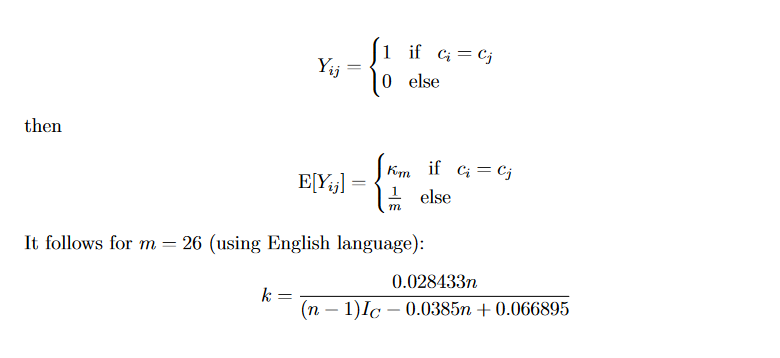
\includegraphics[scale=1]{q2_4_1.png}
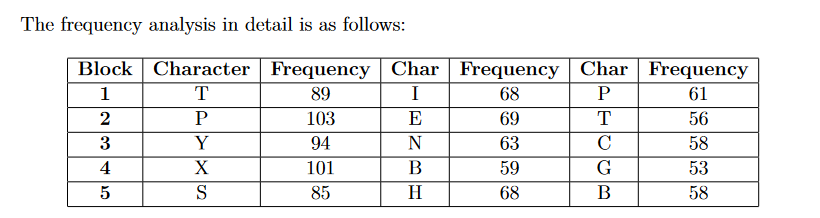
\includegraphics[scale=0.8]{q2_4_2.png}
%%%%%%%%%%%%%%
% Problem 5
%%%%%%%%%%%%%%%%%%%%%%%%%%%%%%%%%%%%%%%%%%%%%%%%%%%%%%%%%%%%%%%%%%%%%%%%%%%%%%%%%%%%%%%%%%%%%%%%%%%%%%%%%%%%%%%%%%%%%%%%%%%%%%%%%%%%%%%%
\begin{problem}{5}
We are given the plain text matrix (P) and the cipher text matrix (C). Therefore, we can solve for the key matrix (K).\\
Plain text matrix (P) x Key matrix (K) = Cipher text matrix (C)\\

Key = [7 19, 8 3]
\end{problem}
\noindent\rule{7in}{2.8pt}
%%%%%%%%%%%%%%%%%%%%%%%%%%%%%%%%%%%%%%%%%%%%%%%%%%%%%%%%%%%%%%%%%%%%%%%%%
%Section 3
%%%%%%%%%%%%%%%%%%%%%%%%%%%%%%%%%%%%%%%%%%%%%%%%%%%%%%%%%%%%%%%%%%%%%%%%%%%%%%%%%%%%%%%%%%%%%%%%%%%%%%%%%%%%%%%%%%%%%%%%%%%%%%%%%%%%%%%%
% Problem 1
%%%%%%%%%%%%%%%%%%%%%%%%%%%%%%%%%%%%%%%%%%%%%%%%%%%%%%%%%%%%%%%%%%%%%%%%%%%%%%%%%%%%%%%%%%%%%%%%%%%%%%%%%%%%%%%%%%%%%%%%%%%%%%%%%%%%%%%%
\section*{Classical Systems - Encrypt}
\begin{problem}{1}
Shift Cipher, also known as Caesar Cipher, is a simple encryption technique that shifts each letter of the plaintext message by a fixed number of positions down the alphabet. It is a type of substitution cipher where each letter in the plaintext is replaced by a letter some fixed number of positions down the alphabet.
Here's some Python code to Encrypt the message:
\lstinputlisting[language=Python, numbers=none]{shift_cipher_encryptor.py}
Shift Cipher = Bpqaqaiamkzmbumaaiom

\end{problem}
%%%%%%%%%%%%%%%%%%%%%%%%%%%%%
% Problem 2
%%%%%%%%%%%%%%%%%%%%%%%%%%%%%%%%%%%%%%%%%%%%%%%%%%%%%%%%%%%%%%%%%%%%%%%%%%%%%%%%%%%%%%%%%%%%%%%%%%%%%%%%%%%%%%%%%%%%%%%%%%%%%%%%%%%%%%%%
\begin{problem}{2}
The Affine cipher is a type of monoalphabetic substitution cipher, where each letter in the plaintext message is replaced by another letter based on a mathematical function. The function used in the Affine cipher is of the form:\\
$E(x) = (ax + b) \% m$\\
where E(x) is the ciphertext letter corresponding to plaintext letter x, a and b are the key values, and m is the size of the alphabet (26 for the English alphabet).\\
To encrypt the message, we first convert it to numerical values using the standard mapping A=0, B=1, C=2, etc.:\\
T H I S I S A S E C R E T M E S S A G E\\
19 7 8 18 8 18 0 18 4 19 2 18 18 0 6 4\\
Then we apply the encryption formula E(x) = (ax + b) mod 26 to each numerical value.\\
Affine Cipher: MEJHJHVHPFCPMDPHHVZP
\end{problem}
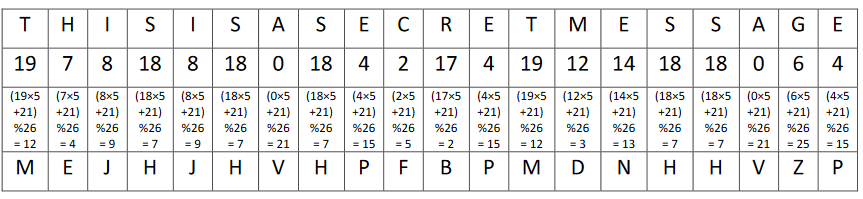
\includegraphics[scale=0.78]{q3_1.png}
%%%%%%%%%%%%%%%%%%%%%%%%%%%%%
% Problem 3
%%%%%%%%%%%%%%%%%%%%%%%%%%%%%%%%%%%%%%%%%%%%%%%%%%%%%%%%%%%%%%%%%%%%%%%%%%%%%%%%%%%%%%%%%%%%%%%%%%%%%%%%%%%%%%%%%%%%%%%%%%%%%%%%%%%%%%%%
\begin{problem}{3}
The Playfair cipher uses a 5x5 grid of letters, where each letter of the alphabet is used except for 'j'. To encrypt a message, the plaintext is divided into pairs of letters and then each pair is encrypted using the rules of the Playfair cipher.\\
Any sensible explanation gets full points
\end{problem}
%%%%%%%%%%%%%%%%%%%%%%%%%%%%%
% Problem 4
%%%%%%%%%%%%%%%%%%%%%%%%%%%%%%%%%%%%%%%%%%%%%%%%%%%%%%%%%%%%%%%%%%%%%%%%%%%%%%%%%%%%%%%%%%%%%%%%%%%%%%%%%%%%%%%%%%%%%%%%%%%%%%%%%%%%%%%%
\begin{problem}{4}
The Vigenere cipher uses a keyword to encrypt a message by shifting each letter of the message by a corresponding amount determined by the letters of the keyword. The key k = (8, 2, 10, 7, 25, 6) indicates the number of positions to shift each letter of the message, with the first letter shifted by 8 positions, the second letter shifted by 2 positions, and so on.\\
Vigenere Cipher: BJSZHYIUOJQKBOOZRHOG
\end{problem}
\noindent\rule{7in}{2.8pt}
%%%%%%%%%%%%%%%%%%%%%%%%%%%%%%%%%%%%%%%%%%%%%%%%%%%%%%%%%%%%%%%%%%%%%%%%%
%Section 4
%%%%%%%%%%%%%%%%%%%%%%%%%%%%%%%%%%%%%%%%%%%%%%%%%%%%%%%%%%%%%%%%%%%%%%%%%%%%%%%%%%%%%%%%%%%%%%%%%%%%%%%%%%%
\section*{Please remember:}
\item That it is important to understand the concepts and techniques behind the solutions provided, rather than simply copying them. If you have any further questions or need additional assistance, feel free to ask. Good luck with your studies!\\
\item Guvf cnegvphyne frpgvba vf rkpyhfviryl vagraqrq sbe bhe zbfg vagryyrpghnyyl tvsgrq fghqragf. Vs lbh jrer noyr gb qrpvcure guvf fragrapr, gura lbh fubhyq or njner gung gur GN grnz ubyqf n terng nccerpvngvba sbe lbh. tvir n fgne gb gur ercbfvgbel bs gur pbhefr naq trg na rkgen obahf sbe purpxvat gur fbyhgvba pnershyyl.
\end{document}
 
% \begin{problem}{2}
% Consider the system
% \begin{align*}
%     x_{k+1} &= \phi x_{k} + w_{k}, \\
%     y_k &= x_k, 
% \end{align*}
% where $w_k \sim (0, 1)$, and $\phi = 0.9$ is an unknown constant. Design an extended Kalman filter to estimate $\phi$. Simulate the filter for $100$ time steps with $x_0 = 1, P_0 = I , \hat{x}_{0} = 0$, and $\hat{\phi}_{0} = 0$. Hand in your source code and a plot showing $\hat{\phi}$ as a function of time.
% \end{problem}
% \begin{solution}
% Perform the measurement update of the state estimate and estimation error covariance as follows
% \begin{align*}
%     K_k &= P^{-}_k H^{\top}_k (H_k P^{-}_k H^{\top}_k + R_k)^{-1} = P^{-}_k H^{\top}_k (H_k P^{-}_k H^{\top}_k)^{-1}, \quad \text{Since }R_k = 0, \\
%     \hat{\bar{x}}^{+}_{k} &= \hat{\bar{x}}^{-}_{k} + K_k (y_k - h_k(\hat{\bar{x}}^{-}_{k}, 0)) \\
%     &= \hat{\bar{x}}^{-}_{k} + K_k (y_k - \hat{x}^{-}_{k}), \quad \text{Since } \hat{\phi}^{-}_{k} = 0, \\
%     P^{+}_k &= (I - K_k H_k) P^{-}_k
% \end{align*}
% \begin{figure}[H]
%     \centering
%     \includegraphics[scale=0.25]{q2.png}
%     \caption{Plot showing $\hat{\phi}$ as a function of time.}
%     \label{fig_q2l}
% \end{figure}
% \end{solution} 
% \lstinputlisting{HW6Q2.m}
% \noindent\rule{7in}{2.8pt}
 